\documentclass[11pt]{article}
\usepackage{epic}
\usepackage{url}
\usepackage{html}

\documentclass[12pt,a4paper,dvips,openright]{article}
%\usepackage{amsmath, amsthm}
\usepackage{theorem}
\usepackage[english]{babel}
%\usepackage{fontenc}
%\usepackage{t1enc}
\usepackage{a4}
\usepackage{epsfig}
\usepackage{amsfonts}
\usepackage{latexsym}
\usepackage{alltt}
\usepackage{url}
\usepackage{color}
\usepackage[normalem]{ulem}
%%\usepackage{html}
%%\usepackage{showlabels}

%\theoremstyle{remark}
\newtheorem{theorem}{Theorem}[section]
\newtheorem{lemma}[theorem]{Lemma}
\newtheorem{proposition}[theorem]{Proposition}
\newtheorem{corollary}[theorem]{Corollary}
\newtheorem{algorithm}[theorem]{Algorithm}
\theorembodyfont{\rmfamily}
\newtheorem{definition}[theorem]{Definition}
\newtheorem{remark}[theorem]{Remark}
\theorembodyfont{\rmfamily}
\newtheorem{example}[theorem]{Example}

\newenvironment{proof}[1][\it Proof.]{\begin{trivlist}\item[\hskip \labelsep {\bfseries #1}]}{$_\Box$\end{trivlist}}





\newcommand{\N}{\ensuremath{\mathbb{N}}}
\newcommand{\Z}{\ensuremath{\mathbb{Z}}}
\newcommand{\Q}{\ensuremath{\mathbb{Q}}}
\newcommand{\R}{\ensuremath{\mathbb{R}}}


\newcommand{\A}{\ensuremath{\mathcal{A}}}
\newcommand{\F}{\ensuremath{\mathcal{F}}}
\newcommand{\G}{\ensuremath{\mathcal{G}}}
\newcommand{\T}{\ensuremath{  \mathcal{T}  }}
\newcommand{\K}{\ensuremath{\mathcal{K}}}
\newcommand{\C}{\ensuremath{\mathcal{C}}}
\newcommand{\CC}{\ensuremath{\mathbb{C}}}

\newcommand{\TT}{\ensuremath{\mathbb{T}}}

%\newcommand{\k}{\ensuremath{{k}}}
%\newcommand{\t}{\ensuremath{{t}}}
\newcommand{\x}{\ensuremath{{x}}}

\newcommand{\init}{\textup{in}}
\newcommand{\tinit}{\textup{t-in}}
\newcommand{\homog}{\textup{homog}}
\newcommand{\spann}{\textup{span}}
\newcommand{\flip}{\textup{flip}}
\newcommand{\face}{\textup{face}}
\newcommand{\supp}{\textup{supp}}
\newcommand{\val}{\textup{val}}
\newcommand{\rank}{\textup{rank}}
\newcommand{\conv}{\textup{conv}}
\newcommand{\minAss}{\textup{minAss}}
\newcommand{\Ass}{\textup{Ass}}
\newcommand{\relint}{\textup{rel int}}
\newcommand{\New}{\textup{New}}
\newcommand{\codim}{\textup{codim}}

\newcommand{\puiseux}{{\ensuremath{\CC\{\{t\}\}} }}


\def\name{Gfan }


\begin{document}
\title{A presentation of the \name software package}
\author{Anders Nedergaard Jensen
\thanks{Partially supported by the Faculty of Science, University of Aarhus, Danish Research Training Council (Forskeruddannelsesr\aa det, FUR) , Institute for Operations Research ETH, grants DMS 0222452 and DMS 0100141 of the U.S. National Science Foundation and the American Institute of Mathematics.
}
\\
\\
\small
Department of Mathematical Sciences, University of Aarhus
and\\
\small
Institute for Operations Research, ETH Z\"urich
}

\maketitle
\begin{abstract}
\name is a new software package for computing Gr\"obner fans of polynomial ideals in $\Q[x_1,\dots,x_n]$.
We give a short description of this package.
Some technical details are given to give the reader an idea of what the software can do.
\end{abstract}


\section{Background}
\begin{description}
\item[Introduction] \name is a software package for computing the \emph{Gr\"obner fan} (\cite{MoRo}) of a given polynomial ideal. It is an implementation of the ideas appearing in \cite{fukuda} which is joint work with Komei Fukuda and Rekha Thomas. For toric and lattice ideals such programs already exist: TiGERS \cite{huber} and CaTS \cite{cats}. \name works on any ideal in $\Q[x_1,\dots,x_n]$. Besides Buchberger's algorithm, the local basis change procedure \cite{collart} and the simplex method, the reverse search technique \cite{avis} and algorithms for exploiting symmetry are used. This allows enumeration of fans with millions of cones. \name has been used for studying the structure of the Gr\"obner fan. Among the new results is an example of a Gr\"obner fan which is not the normal fan of a polyhedron \cite{jensen}.
\item[The Gr\"obner fan of an ideal] The Gr\"obner fan of an ideal $I\subset k[x_1,\dots,x_n]$ is a polyhedral complex consisting of cones in $\R^n$. The monomial initial ideals (with respect to term orders) of $I$ are in bijection with the marked reduced Gr\"obner bases of $I$ and with the full dimensional cones in the Gr\"obner fan of $I$. Knowing a marked reduced Gr\"obner basis its initial ideal and equations defining its Gr\"obner cone are easily read off. Thus a useful way to present the Gr\"obner fan of an ideal is by the set of its reduced Gr\"obner bases.
\end{description}
\section{Demonstration of the software}
\begin{description}
\item[Computing all re\-duced Gr\"obner bases] \hspace{0.2cm} Computing all reduced Gr\"obner bases of a polynomial ideal is the primary purpose of the software. This can be done using the program {\tt gfan}. For example, running
\begin{verbatim}
gfan
\end{verbatim}
on the input
\begin{verbatim}
{a^2+b*c, b^2+a*c, c^2+a*b}
\end{verbatim}
produces a list of the 9 reduced Gr\"obner bases of the ideal generated by the input:
\begin{verbatim}
{{c^4, b*c^2, b^2*c, b^3-c^3, a*c+b^2, a*b+c^2, a^2+b*c},
{c^3-b^3, b*c^2, b^2*c, b^4, a*c+b^2, a*b+c^2, a^2+b*c},
{c^2+a*b, b^2*c, b^4, a*c+b^2, a*b^2, a^2+b*c},
{c^2+a*b, b*c+a^2, b^4, a*c+b^2, a*b^2, a^2*b, a^3-b^3},
{c^2+a*b, b*c+a^2, b^3-a^3, a*c+b^2, a*b^2, a^2*b, a^4},
{c^4, b*c^2, b^2+a*c, a*c^2, a*b+c^2, a^2+b*c},
{c^4, b*c+a^2, b^2+a*c, a*c^2, a*b+c^2, a^2*c, a^3-c^3},
{c^3-a^3, b*c+a^2, b^2+a*c, a*c^2, a*b+c^2, a^2*c, a^4},
{c^2+a*b, b*c+a^2, b^2+a*c, a^2*c, a^2*b, a^4}}
\end{verbatim}
\item[Combining programs on the command line]
Since \name is not part of a big algebra program we are limited to doing manipulations supported by the UNIX shell. The \name package contains other programs than {\tt gfan}. For example we may combine {\tt gfan} and {\tt gfan\_polynomialsetunion} using the pipe operation to compute a \emph{universal} Gr\"obner basis:
\begin{verbatim}
gfan | gfan_polynomialsetunion
\end{verbatim}
With the same input as before the output will be
\begin{verbatim}
{c^4, b*c^2, b^2*c, b^3-c^3, a*c+b^2, a*b+c^2,
a^2+b*c, c^3-b^3, b^4, a*b^2, a^2*b, a^3-b^3,
b^3-a^3, a^4, a*c^2, a^2*c, a^3-c^3, c^3-a^3}
\end{verbatim}
Another possibility is to visualize the Gr\"obner fan.
\begin{verbatim}
gfan | gfan_render > picture1.fig
\end{verbatim}
will produce the first xfig file shown in Figure \ref{fig:fan} while the following will render the staircase diagrams:
\begin{verbatim}
gfan | gfan_renderstaircase -m > picture2.fig
\end{verbatim}

\begin{figure}
\begin{center}
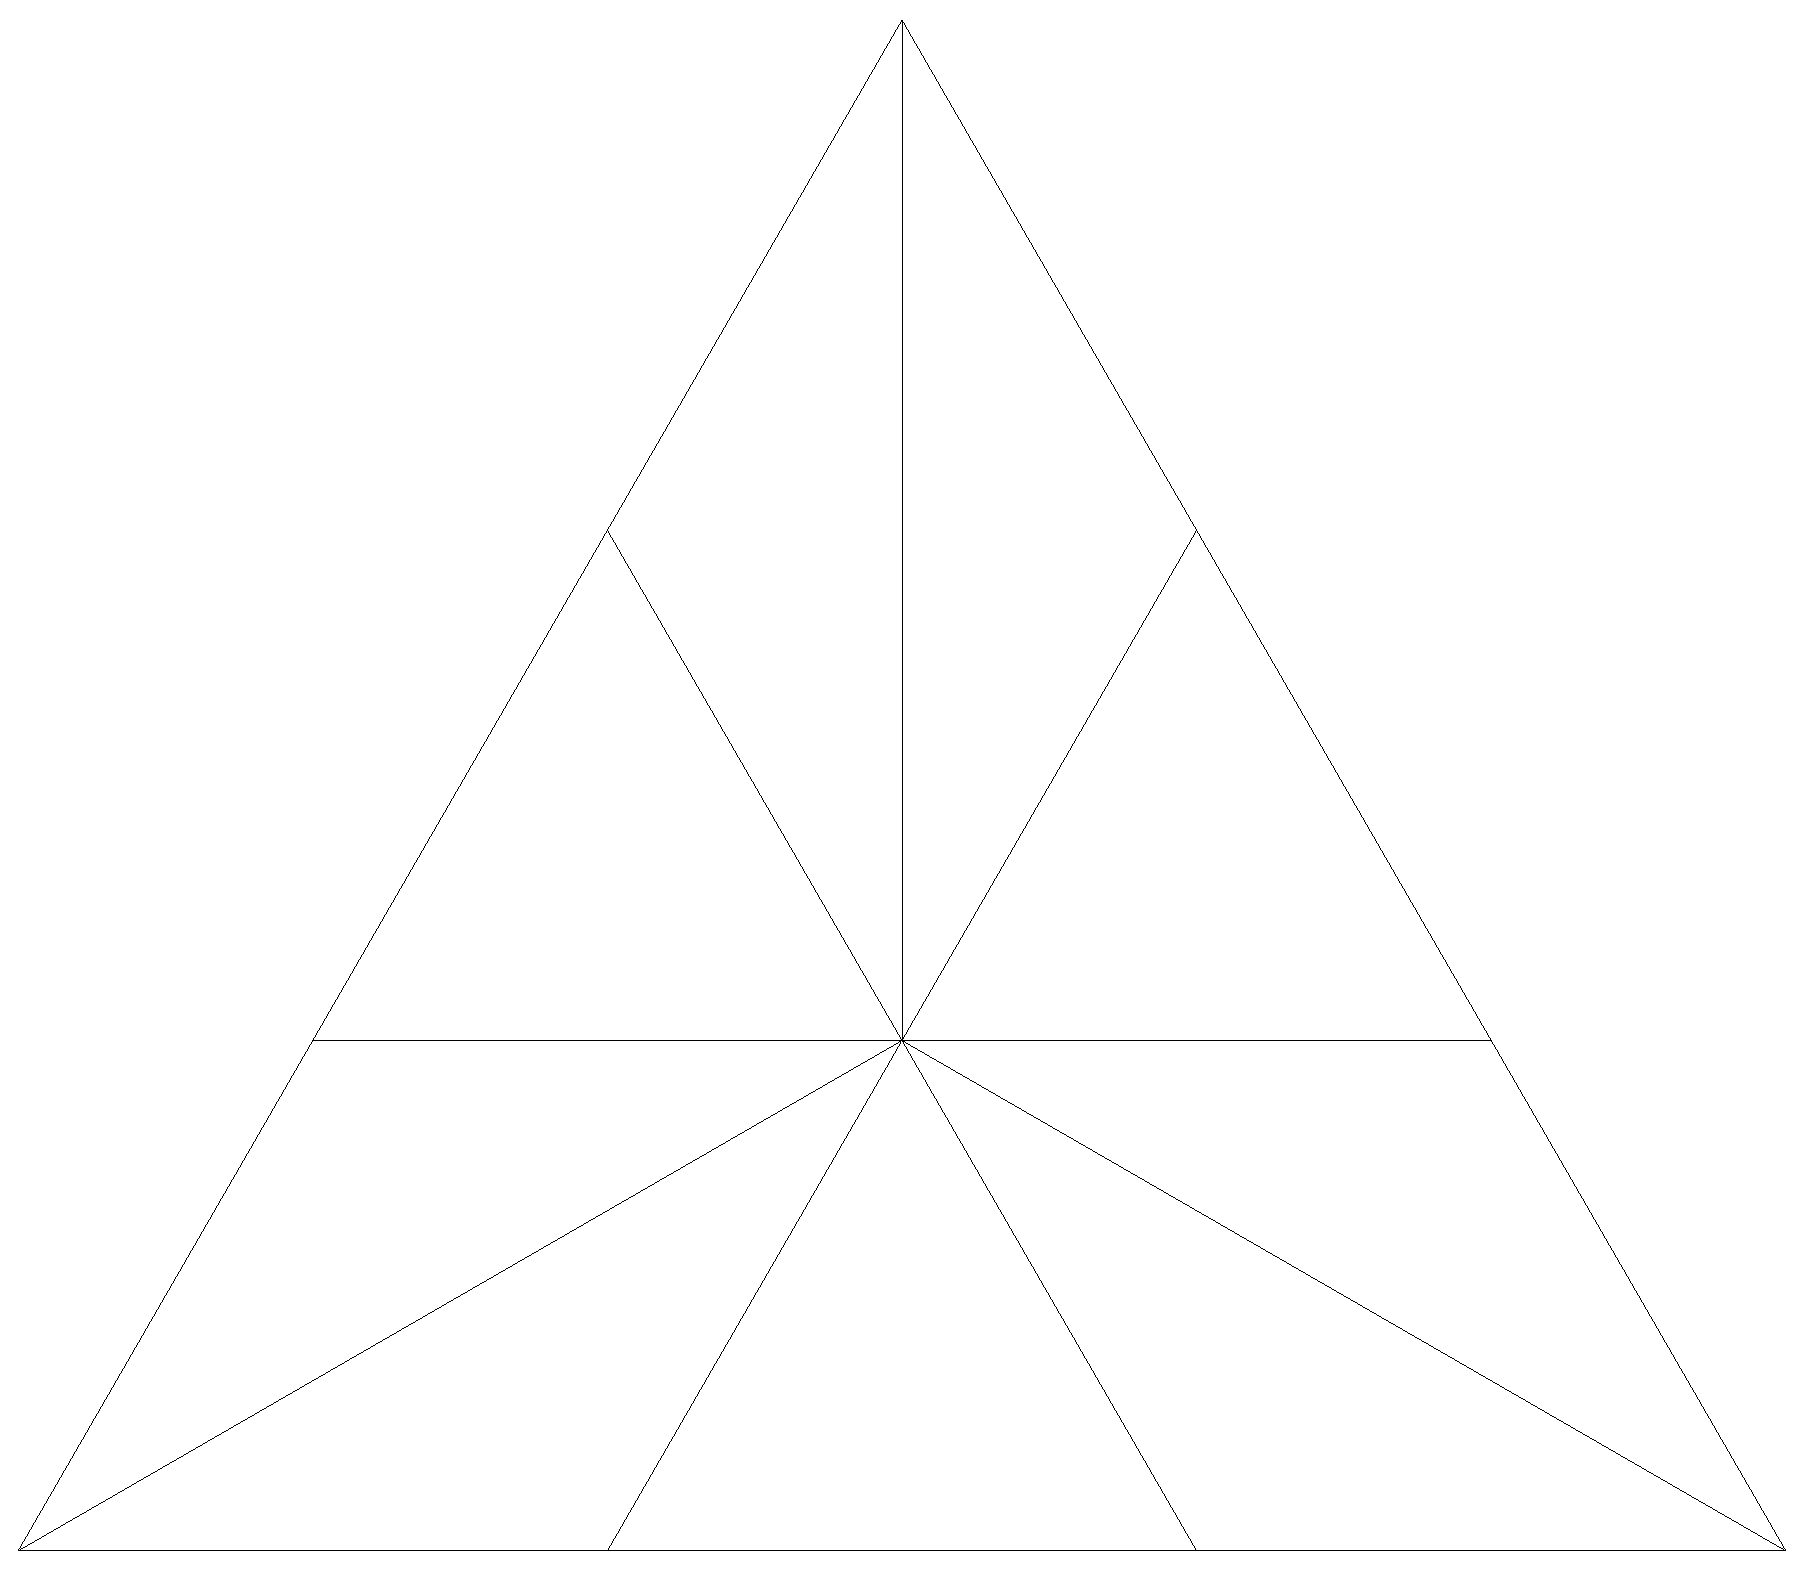
\epsfig{file=gfan1.eps,height=3.9cm} 
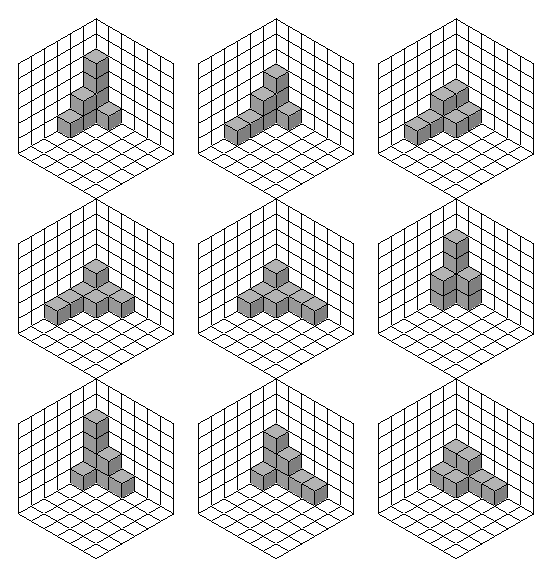
\epsfig{file=staircase.eps,height=3.9cm} 
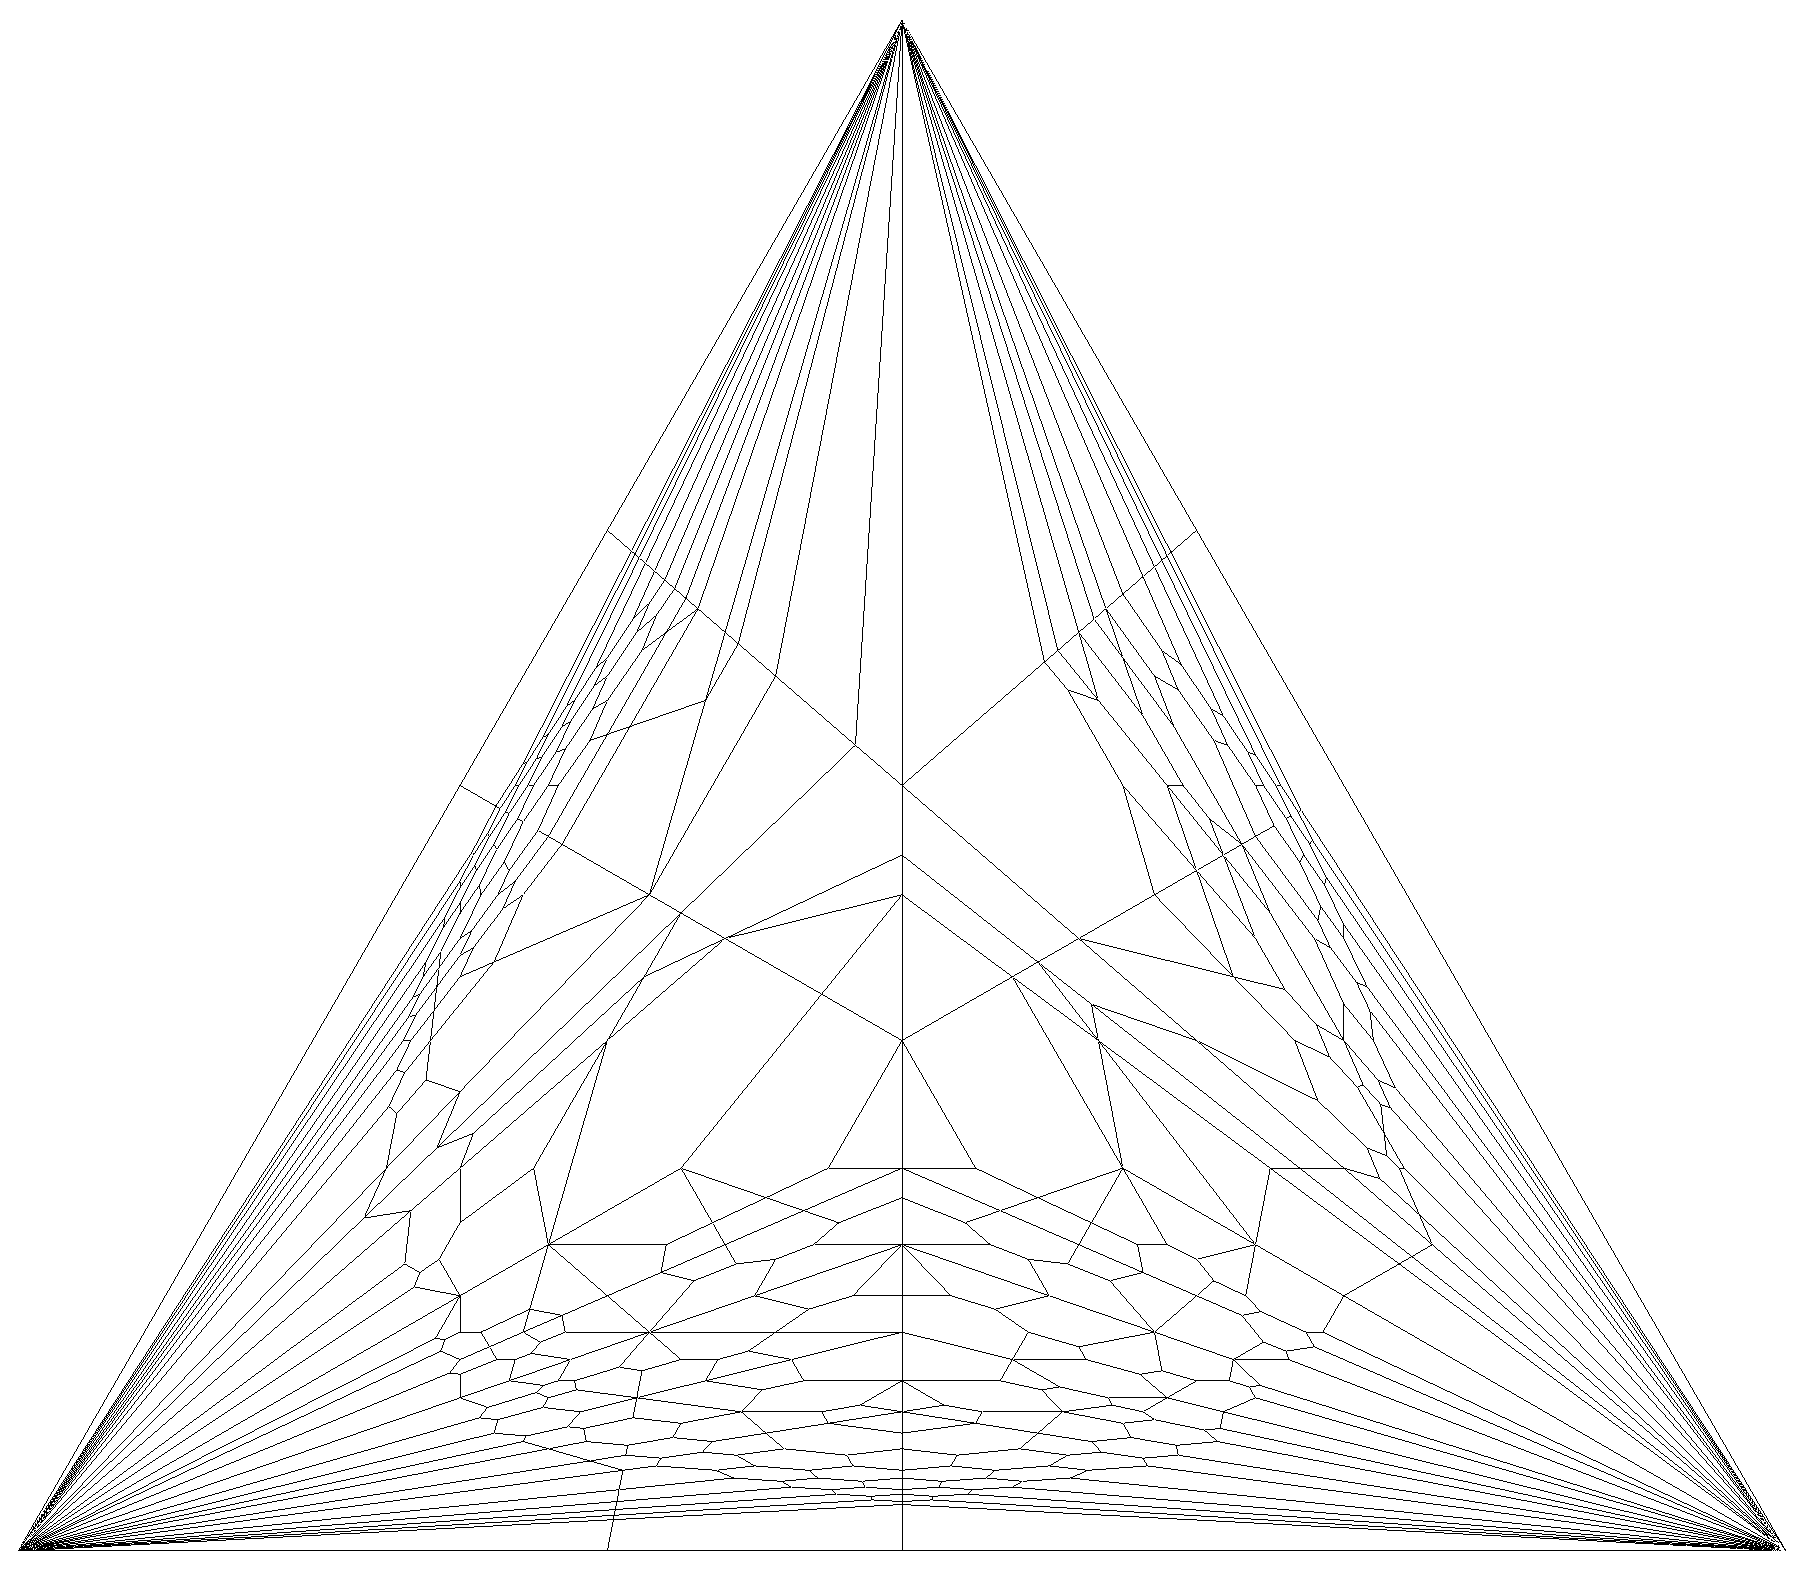
\epsfig{file=gfan2.eps,height=3.9cm} 
\end{center}
\caption{The Gr\"obner fan of the ideal intersected with the standard simplex, staircase diagrams visualising the various monomial initial ideals and a Gr\"obner fan of a different ideal.}
\label{fig:fan}
\end{figure}

\end{description}
\section{Advanced features}
\begin{description}
\item[Symmetry] Our examples are rarely random. They often possess a lot of symmetry. In our example, the ideal is invariant under any permutation of the three variables. In many cases it would be sufficient to know only the essentially different Gr\"obner bases. \name can do its computations up to symmetry.
\item[Interactive mode] The program {\tt gfan\_interactive} is useful for investigating the local structure of the fan. It allows the user to interactively walk from cone to cone along an arbitrary path in the Gr\"obner fan.
\end{description}
\section{Final remarks}
\begin{description}
\item[Performance] The software has been used to compute big examples. Here is an example of its performance: The ideal generated by the $4\times 4$ minors of $4\times 5$ matrix has 3000 reduced Gr\"obner bases. They can be computed in 5 hours using reverse search. Exploiting the symmetry of the ideal they can be computed in 12 seconds.
\item[Future improvements] A natural extension of the software is a program for checking if a set of polynomials is a Gr\"obner basis with respect to \emph{some} (unknown) term order. Another could be a \emph{universal} Gr\"obner basis test - is a given set of polynomials a Gr\"obner basis with respect to \emph{any} term order?
\item[Supported platforms and required libraries] The following platforms are supported: Linux, Mac OS X and other UNIX variants. It is likely that the program will also run on Microsoft Windows systems through Cygwin. The program is written in C++ and can be compiled with gcc 3.3.3. The following libraries are required: gmp \cite{gmp} (arithmetics) and cddlib \cite{cdd} (LP-solving).
\end{description}

\bibliographystyle {plain}
\bibliography{jensen.bib}
 
\end{document}
